%%%%%%%%%%%%%%%%%%%%%%%%%%%%%%%%%%%%%%%%%%%%%%%%%%%%%%%%%%%%%%%%%%%%%%%%%%
% Current i_1a(wt)
%%%%%%%%%%%%%%%%%%%%%%%%%%%%%%%%%%%%%%%%%%%%%%%%%%%%%%%%%%%%%%%%%%%%%%%%%%
\begin{solutionfigure}[htb]

    %   \documentclass{standalone}
    %   \usepackage{pgfplots}
    %   \pgfplotsset{compat=1.18} % Kompatibilität für neuere Versionen
           \centering
           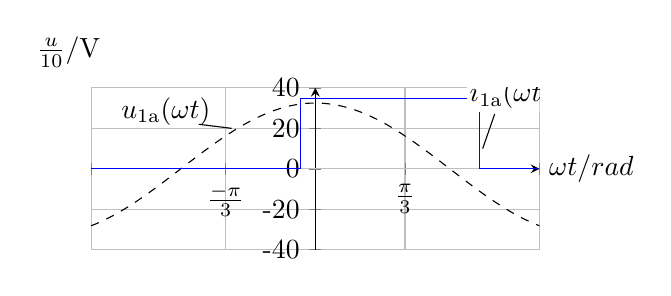
\begin{tikzpicture}
               \begin{axis}[
                   % x/y range adjustment
                   xmin=-150, xmax=150,
                   ymin=-40, ymax=40,
                   samples=500,
                   axis y line=center,
                   axis x line=middle,
                   extra y ticks=0,
                   % Label text
                   xlabel={$\omega t / \text{rad}$},,
                   ylabel={$\frac{u}{10}/\mathrm{V}$},
                   % Label adjustment
                   x label style={at={(axis description cs:1,0.5)},anchor=west},
                   y label style={at={(axis description cs:-.05,.97)},anchor=south,yshift=0.2cm},
                   width=0.6\textwidth,
                   height=0.3\textwidth,
                   % x-Ticks
                   xtick={-150,-60,0,60,150},
                   xticklabels={,$\frac{-\pi}{3}$,0,$\frac{\pi}{3}$,,},
                   xticklabel style = {anchor=north},
                   % y-Ticks
                   ytick={40,20,0,-20,-40},
                   yticklabels={40,20,0,-20,-40},
                   yticklabel style = {anchor=east},
                   % Grid layout
                   grid,
                   %grid style={line width=.1pt, draw=gray!10},
                   %major grid style={line width=.2pt,draw=gray!90},
               ]
               % Voltage u1a(wt)
               \addplot[black, domain= -150:150,dashed] {32.5*cos(x)};
                % Current i1a(wt)
               \addplot[color=blue,solid] coordinates{
                (-150,0)
                (-10.09, 0)
            };                 
               \addplot[color=blue,solid] coordinates{
                (-10.09,0)
                (-10.09, 34.6)
            };                   
               \addplot[color=blue,solid] coordinates{
                   (-10.09,34.6)
                   (109.9, 34.6)
               };  
               \addplot[color=blue,solid] coordinates{
                (109.9,0)
                (109.9, 34.6)
            };
            \addplot[color=blue,solid] coordinates{
                (109.9,0)
                (150, 0)
            };    
               % Label of i1a
               \node[black, fill=white, inner sep = 1pt, anchor = south] at (axis cs:131,28) {$i_{\mathrm{1a}}(\omega t)$};
                % Label of u1a           
               \node[black, fill=white, inner sep = 1pt, anchor = south] at (axis cs:-100,20) {$u_{\mathrm{1a}}(\omega t)$}; 
               % Line for u1a
               \draw[thin, black] (-78,22) -- (-56,20);
               % Line to i1a
               \draw[thin, black] (112,10) -- (120,27);
           \end{axis}     
           \end{tikzpicture}
           \caption{Input Current $i_\mathrm{1a}(\omega t)$}
           \label{sfig:ex06_current_signals_6_1_4a}
   \end{solutionfigure}